\documentclass[../Main/Main.tex]{subfiles}

\begin{document}
Como base fundamental de este trabajo, a continuación, se expondrá a detalle el modelo. El objetivo, es construir un clasificador binario flexible con buena fuerza predictiva. La notación se irá explicando conforme aparece pero existe un compendio en el Apéndice \ref{ap:Notacion}. En general, se trata de respetar la notación que usan en los libros \autocite{hastie2008elements} y \autocite{james2013introduction}\\

Se supone la siguiente estructura en los datos:
\begin{itemize}
	\item $\{(y_i,\xni)\}_{i = 1}^n$ con $n$ el tamaño de la muestra.
	\item $y_i \in \{0,1\}\quad \forall i = 1\ldots,n$  variables de respuesta binarias o \textit{output}.
	\item $\xni \in \mathcal{X}^d \subseteq \mathbb{R}^d \quad \forall \; i = 1\ldots,n$ covariables, regresores o \textit{input}.
	\item $d \in \mathbb{N}$ dimensionalidad de las covariables.
\end{itemize}

El modelo en si, se presenta a continuación de forma general para cualquier pareja de datos $(y,\xsn)$:
\begin{align}
y\,|\,z\, &\sim \text{Be}(y\,|\Phi(z)) \label{ec:Y-Z} \\ 
z\,|\,x\, &\sim \text{N}(z\,|f(\xsn),1) \label{ec:Z-X}\\
f(\xsn) &\approx \sum_{j=0}^d \beta_j f_j(x_j) \label{ec:fproy} \\[4pt]
f_j(x_j) &\approx \sum_{l = 1}^{\N} w_{j,l} \Psi_{j,l}(x_j, \mathcal{P}_j) \quad \forall j= 0,1,\ldots,d \label{ec:fj}
\end{align}	
En las expresiones (\ref{ec:Y-Z}) y (\ref{ec:fproy}), dejando de un lado ecuación (\ref{ec:Z-X}), se tiene una versión ligeramente modificada de un GLM (Sec. \ref{sec:GLM}). Esto, pues la variable de respuesta $y$ es binaria modelada con una distribución Bernoulli. Además, (\ref{ec:fproy}) es una función de proyección lineal como las que se usan el los modelos tradicionales. En el contexto de un modelo probit, esta función $f$, busca separar el espacio $d$-dimensional de covariables $\mathcal{X}^d$ en regiones identificables en una sola dimensión $\mathbb{R}$. Esta función de proyección, asume que la dependencia entre covariables se puede modelar como la suma ponderada de los componentes $f_j$ (Sec. \ref{sec:FuncProy}). Para poder hacer la liga entre ambas ecuaciones, se requiere de la incorporación de una variable latente $z$, vista en la ecuación (\ref{ec:Z-X}), esta variable es meramente estructural y será modelada a través de una distribución normal, lo cual lleva a tener un modelo probit. Finalmente (\ref{ec:fj}) hace una transformación no lineal de cada dimensión $j$ y trata de encontrar las tendencias individuales de cada una de las covariables. Esto se logra, haciendo un suavizamiento por medio de polinomios por partes que dependen de 3 objetos: una partición del intervalo $\P_j$, un vector de pesos $w_j$ y parámetros que captura la $\N$ especificando la forma y grado de los polinomios. La forma funcional de $\Psi$ es compleja y relativamente arbitraria dependiendo de la selección de la base, por lo tanto, no se especifican aún y se deja para la Sección \ref{sec:fj}. Se hace notar que el componente bayesiano se explora hasta el Capítulo \ref{cap:BayesAlgoritmo} pues va estrechamente ligado con su implementación.  En la Figura \ref{fig:DiagramaMod} se hace una representación visual del modelo para su mejor comprensión.

% Diagrama del modelo
\begin{figure}[h] 
\centering
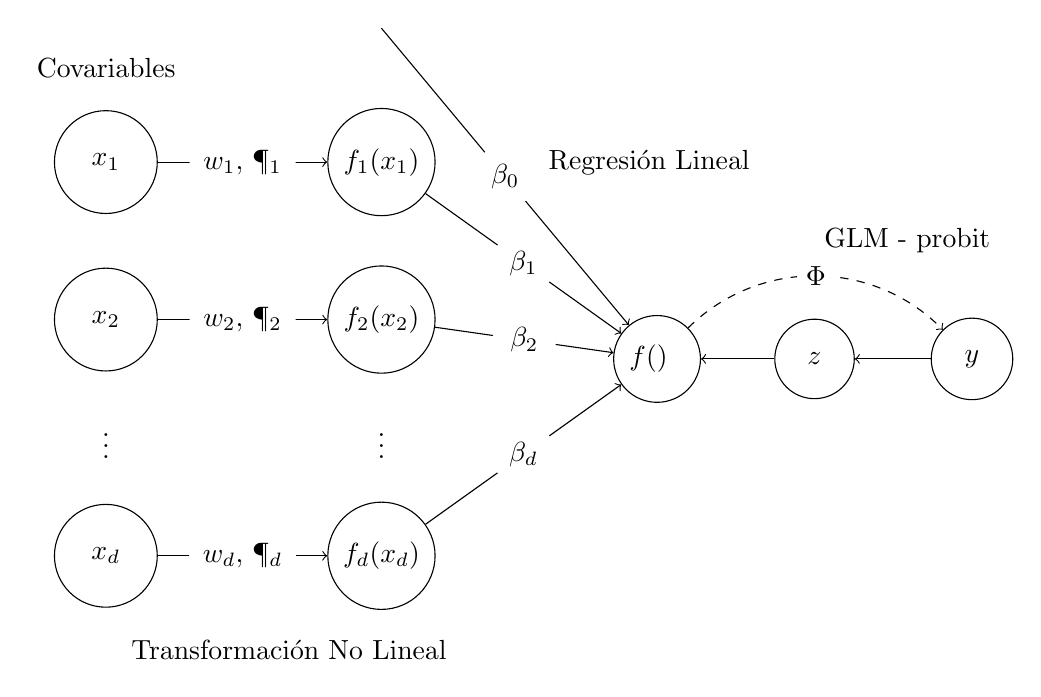
\begin{tikzpicture}

% Nodos Input
\begin{scope}[
		every node/.style = {shape = circle, draw = black,
			minimum size = 10mm,
			text width = 10mm, align = center}]
	\node (x1) at (0,6) {$x_1$};
	\node (x2) at (0,4) {$x_2$};
	\node[draw = white]     at (0,2.5) {$\vdots$};
	\node (xd) at (0,1) {$x_d$};

% Nodos Segunda Capa
	\node (f1) at (3.5,6) {$f_1(x_1)$};
	\node (f2) at (3.5,4) {$f_2(x_2)$};
	\node[draw = white]     at (3.5,2.5) {$\vdots$};
	\node (fd) at (3.5,1) {$f_d(x_d)$};
\end{scope}

% Nodos Lineales
\begin{scope}[
		every node/.style = {shape = circle, draw = black,
			minimum size = 7mm,
			text width = 7mm, align = center}]
\node (f) at (7,3.5) {$f(\xsn)\quad$};
\node (z) at (9,3.5) {$z$};
\node (y) at (11,3.5) {$y$};
\end{scope}

% Nodos Texto 

\node[right] at (-1,7.2) {Covariables};
\node[right] at (0.2,-0.2) {Transformación No Lineal};
\node[right] at (5.5,6) {Regresión Lineal};
\node[right] at (9,5) {GLM - probit};

% Pahts x a f_j y f_j a f
\begin{scope}[
		every node/.style={fill = white, circle},
	    every edge/.style={draw = black, ->}]
	 
	% Paths x a f_j
	\path (x1) edge node {$w_1, \, \P_1$} (f1);
	\path (x2) edge node {$w_2, \, \P_2$} (f2);
	\path (xd) edge node {$w_d, \, \P_d$} (fd);

	% Paths f_j a f
	\path (3.5,7.7) edge node {$\beta_0$} (f);	
	\path (f1) edge node {$\beta_1$} (f);
	\path (f2) edge node {$\beta_2$} (f);
	\path (fd) edge node {$\beta_d$} (f);
\end{scope}

% Ultimos Paths
	\path[->, dashed] (f) edge [bend left = 45]
	node [fill = white] {$\Phi$}(y);	
	\draw[->] (y) -- (z);	
	\draw[->] (z) -- (f);

\end{tikzpicture}
\caption{\textbf{Diagrama del modelo.} Se hace una transformación no lineal de las covariables $x_j$ a través de los parámetros $w_j$ y $P_j$. Con los datos transformados $f_j$, se lleva a cabo un modelo probit con función liga $\Psi$ para lograr la clasificación binaria en $y$.}
\label{fig:DiagramaMod}
\end{figure}

Antes de continuar, vale la pena recordar que:
\begin{quote}
\textit{All models are wrong but some are useful}\footnote{\autocite{box1979robustnessinthe}}
\end{quote}

Escoger un modelo que explique perfectamente los datos o que logre predecir todo sería una tarea inútil. Sin embargo, no significa que no se pueda intentar discernir un patrón y es justamente lo que se busca con la construcción de este modelo. Además de entender a profundidad un modelo que sirve como base para modelos que se están usando en el mundo de la inteligencia artificial. En particular, este modelo tiene la ventaja que es flexible y, al menos en teoría, debería de servir para representar una gran cantidad de datos.

\section{Modelos Lineales Generalizados (GLM)} \label{sec:GLM}
Los modelos lineales generalizados, \autocite{sundberg2016exponential} y \autocite{maccullagh1989generalized}, surgen como una generalización del modelo lineal ordinario $y = \beta^tx + \epsilon$ donde $y \in\mathbb{R}$. En esta generalización, se busca darle otros rangos a $y$ pues se tienen casos donde está restringida a un subconjunto de los reales como lo es el caso binario. Sin embargo, este cambio vuelve el modelo más complejo y lleva a técnicas diferentes en la estimación de los parámetros $\beta$. Además, se pierde algo de la interpretabiliad del modelo\footnote{Dependiendo de la especificación, su interpretación puede ser complicada. Por ejemplo, cuando se tiene un modelo logit tradicional, se logra expresar el logaritmo de la proporción de probabilidades (\textit{Log-Odds-Ratio}) como una combinación lineal de las covariables. $\ln(\pi_i / \pi_0) = \beta^t x$}. Sin embargo, han resultado ser realmente útiles. \\

Los GLM se especifican (de manera muy general) de la siguiente manera:
\begin{align} 
	y &\sim F(\theta(x)) \label{ec:GLM} \\ 
	z &= \beta^tx \nonumber \\ 
	\theta &= g^{-1}(z) \nonumber
\end{align}
con los siguientes tres elementos:

\begin{enumerate}
	\item $F$: \textbf{Tipo de distribución} de la familia exponencial que describa el dominio de las respuestas $y$. Por ejemplo: Bernoulli si $y$ es binaria, Poisson si $y \in \mathbb{Z}^+$ o una distribución Gamma si $y \in \mathbb{R}^+$
	\item $z$: \textbf{Proyector lineal} que explique (linealmente) la variabilidad sistemática de tus datos. En el modelo tradicional $\text{dim}(\beta) = d < n.$
	\item $g$: \textbf{Función liga} que una la media (o los parámetros canónicos) $\theta$ de mi distribución con el proyector lineal. Es decir: $\theta(x) = \E[y|x] = g^{-1}(\beta^tx)$. 
	
	Como ejemplos clásicos se tiene la función $\text{logit}(p) = \ln(p/(1-p))$ o la $\text{probit(p)} = \Phi^{-1}(p)$, donde $p = \E[y|x]$ y $\Phi(\cdot)$ la función de acumulación de una distribución normal estándar. En la Figura \ref{fig:DiagramaFuncLiga} se puede ver una representación gráfica para su mejor comprensión.
\end{enumerate}

% Diagrama de g
\begin{figure}[h]
\centering
\begin{tikzpicture}

% Flechas (circulo) (Solo para demostrar que el orden importa en rikz
%\draw [black] (0,0) circle [radius = 2];

% Dibujo nodos
\begin{scope}[
		every node/.style = {fill = white, shape = rectangle }]
		
	\node (g) at (0,1) {$g$};
	\node (ginv) at (0,-1) {$g^{-1}$};
	\node (R) at (1,0) {$\mathbb{R}$};
	\node (int) at (-1,0) {$[0,1]$};
	
\end{scope}

% Flechitas
\begin{scope}[
		every node/.style={fill = white, circle},
	    every edge/.style={draw = black, ->}]
	
	\path (g) edge [bend left] node [above right] 
	{e.g. $\Phi^{-1}(p)$} (R);
	\path (R) edge [bend left] node [below right] {x} (ginv);
	\path (ginv) edge [bend left] node [below left]
	{e.g. $\Phi(x)$} (int);
	\path (int) edge [bend left] node [above left] {p} (g);
	
\end{scope}

\end{tikzpicture}
\caption{\textbf{Esquema de función liga $g$}}
\label{fig:DiagramaFuncLiga}
\end{figure}

Para este trabajo, se busca construir un clasificador binario por lo que $y \in \{0,1\}$, por lo cual, es natural modelar $y$ como una distribución Bernoulli. Notese que si $Y \sim \Be(y|p)$ se tienen las siguientes propiedades: 
\begin{align*}
	\E[Y] &= p = P(y = 1) \\
	\Var[Y] &= p(1-p)
\end{align*}
Por lo que solo se tiene un parámetro $p$ y la varianza queda determinada automáticamente. Además, esta especificación deja como  opción para las función liga, a las inversas de las funciones \textit{sigmoidales} $s(x)$. Las funciones sigmoidales, son funciones $s:\mathbb{R}\rightarrow (0,1)$, estrictamente monótonas y por ende, biyectivas. Algunos ejemplos son las ya mencionadas logit, probit y la curva de Gompertz\footnote{Para no caer en redundancia de notación para este trabajo se tiene a partir de ahora: $s(x) = g^{-1}(x) = \Phi(x)$}. Estas funciones cumplen un papel de activación, es decir, una vez que se rebase cierto umbral, crecen rápidamente y toman valores más cercanos a uno, \textit{activando} asi la probabilidad de que $y$ sea un éxito. \footnote{En un contexto de redes neuronales, lo que se activa es la neurona y recientemente, se usa la función \textit{ReLu} $(x):= \max\left\{0,x\right\}$}. Esto las hace perfectas herramientas para ligar el proyector lineal $z\in\mathbb{R}$ con una probabilidad $p\in[0,1]$.\\

\subsection{Uso de la Variable Latente}

Ahora, para entender el papel que juega $z$, se necesita entender que es posible estructurar estos modelos como \textit{modelos de variable latente} \autocite{albert1993bayesian}. Bajo esta formulación, se asume que la relación entre $y$ y $x$ no es directa, sin embargo, existe una variable no observada $z$ estructural que ayuda a discernir un vínculo entre ellas. En la Figura \ref{fig:DiagramaVar} se tiene una representación gráfica de esto. \\

%Diagrama de Variable latente
\begin{figure}[h]
\centering
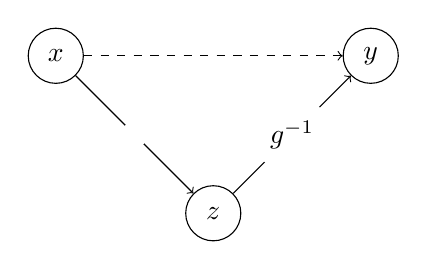
\begin{tikzpicture}

% Nodos Input
\begin{scope}[
		every node/.style = {shape = circle, 
		draw = black, minimum size = .7cm}]
	\node (X) at (0,2) {$x$};
	\node (Y) at (4,2) {$y$};
	\node (Z) at (2,0) {$z$};
\end{scope}

% Paths
\begin{scope}[
		every node/.style={fill = white, circle},
	    every edge/.style={draw = black, ->}]
	\path (X) edge node {} (Z);
	\path (Z) edge node {$g^{-1}$} (Y);
	\draw[dashed, ->] (X) to (Y);
\end{scope}
\end{tikzpicture}
\caption{\textbf{Modelo de variable latente}}
\label{fig:DiagramaVar}
\end{figure}

Tradicionalmente, la normalidad en $z$ es derivada de asumir normalidad en los errores; es decir, dada la regresión lineal $z = \beta^tx + e$ se asume (y se debe verificar) que $e \sim N(0,\sigma^2)$. Lo cual lleva a $z \sim N(\beta^tx,\sigma^2)$. Además este supuesto facilita la estructura de los modelos y el algoritmo de ajuste. Bajo un paradigma frequentista, la estimación de los parámetros $\beta$ se reduce a encontrar los estimadores de mínimos cuadrados. Sin embargo, bajo el paradigma bayesiano, dentro de un modelo probit como el de este trabajo, se adopta la normalidad en $z$ pues en  \autocite{albert1993bayesian}, se sugiere un algoritmo \textit{Gibbs sampler} con distribuciones truncadas de la normal para encontrar $\beta$.\\

La función liga probit se escoge como consecuencia de la normalidad en $z$, o viceversa, dependiendo de como se quiera ver. Esta función $\Phi^{-1}(p)$ es la inversa de la función de acumulación normal estándar:
$$\Phi(x) = \int_{-\infty}^x \dfrac{1}{\sqrt{2\pi}}e^{-\frac{t^2}{2}}\, dt$$
la cual no tiene forma cerrada. Sin embargo, tiene justamente las propiedades que se necesitan pues es claramente sigmoide. Esta función, cumple el propósito de modelar y cuantificar la incertidumbre pues está transformando la variable real $z$ en una probabilidad $p$ con su característica forma de ``s''. Se hace notar que se podría haber usado una función más flexible o que incluso se podría dejar la función como una parte del modelo a estimar. Sin embargo, al adoptar el algoritmo antes citado, se requiere esta especificación.\footnote{En modelos multinomiales bayesianos, tomar esta decisión estructural lleva a que inclusive, se puede asumir una estructura de interdependencia en los errores aleatorios. $\mathbf{e} ~ N_k(0, \Sigma)$ con $\Sigma$ una matriz de correlaciones}. La parte flexible de este modelo se encuentra en el proyector lineal. \\

Habiendo definido la función liga, distinguir entre si $y = 1$ ó 0, éxito o fracaso respectivamente, se reduce a distinguir en que área del espacio de covariables $\mathcal{X}^d$ se encuentra el dato. Esto se debe a que $y = 1$ cuando $\Phi(z) > 1/2$ que sucede \textit{si y solo si} $z>0$ lo cual, depende en gran media de su media; en este caso la función de proyección $f(\xsn)$. Si esta función es muy positiva en alguna región, implicará que el modelo tiene mucha evidencia para confiar que, al menos en esa área, la respuesta $y$ es un éxito. El razonamiento, funciona de forma análoga para los casos donde $y = 0$, claramente, para esas regiones, se busca que $f(\xsn)$ sea negativa. Por lo tanto, es fundamental para el modelo que se realice una correcta estimación de los parámetros de la función de proyección.  Nótese además, que $z$ le agrega cierta \textit{estocasticidad} al modelo. Bajo la suposición que existe una pareja $(y_i,\xni)$ tal que $f(\xni) = 0$; alrededor de una vecindad de este punto, no se tendría evidencia para clasificar a $y_i$ como un éxito o como un fracaso; sería mejor un volado.\\ 

Otro factor importante a considerar, es que el modelo asume que la varianza de $z$ es constante, específicamente $\sigma^2 = 1$. Dado que la escala de $z$ es completamente arbitraria pues es una variable auxiliar, se puede \textit{restringir} $z$ al rango que se desee. El método de simulación para $z$ usando una distribución normal truncada se simplifica ligeramente usando esta varianza unitaria. Se verá en los resultados, sin embargo, que dada la naturaleza global de los polinomios que se usan, la escala de $z$, o al menos la estimación de su media $\hat{f}(\xsn)$, puede variar mucho dependiendo de los datos, mas esto no representa un problema. Pues, en la practica, al  usar el algoritmo de Albert y Chibb $z$ sirve mucho más, para hacer la ligadura de $y$ hacia $f$ y no viceversa. En $z$ se codifica, mediante una normal truncada, los casos de éxito y de fracasos de $y$; posteriormente, se estima el vector $\beta$ para la función $f$. Por ello, en la Figura (\ref{fig:DiagramaMod}), se representan las flechas de $y$ a $f$ por medio de $z$ y solidas, en contraposición con la flecha punteada que va, directamente de $f$ a $y$ y pasa por la función $\Phi$. Los detalles y su justificación probabilista, se tocan en detalle en el Capítulo \ref{cap:BayesAlgoritmo}.\\

% REVISAR
% Probar (o buscar la prueba de este resultado)
Es importante mencionar, que el \textit{corte} que se hace en $z = 0$ para la clasificación, es resultado de hacer una clasificación binaria. En modelos multinomiales también se debe tomar en cuenta los intervalos en $\mathbb{R}$ para los que la observación se clasificaría en alguna de las posibles clases y por ende, estimar los umbrales o usar una función diferente a las sigmoides. Este hecho, lleva a la realización de que $z$ y su media $f$ son \textit{ajenas más no independientes}. Esto quiere decir que la parametrización de $z$ como una normal $N(\mu,1)$ es equivalente a la parametrización $N(0,1)$. Este hecho se hará más claro cuando se hable del papel de $\beta_0$ en la función de proyección. \\ 

Finalmente, si se quisiera ver la relación de $x$ en $y$ directamente, se puede lograr usando el teorema de la probabilidad total. Se puede calcular (al menos de forma teórica), la distribución marginal de $y$ dado $\xsn$ sumando sobre $z$:
% REVISAR - Integral en libro de Cox
\begin{align*}
P(y|x) 	&= \intinfty P(y|z)P(z|x)\, dz \\
		&= \intinfty p(y;\Phi(z))p(z;f(\xsn),\sigma^2)\, dz \\
		&= \intinfty \Phi(z)^y (1-\Phi(z))^{1-y}
		\dfrac{1}{\sqrt{2\pi\sigma^2}}e^{-\frac{1}{2\sigma^2}(z-f(\xsn))^2} \, dz
\end{align*}
Sin embargo, está claro que esta derivación no lleva a ningún resultado analítico cerrado pues la relación es bastante más compleja como para resultar en una distribución  tradicional; si lo hiciera, el propósito de la $z$ se perdería.\\

Recapitulando, mediante la función liga $\Phi$ se une la media $p$, la probabilidad de éxito o fracaso, de la respuesta $y$ con los datos $\xsn$. Esto se logra, a través de una variable auxiliar $z$ cuya media $f(\xsn)$ es una función de proyección lineal. 
\begin{align} \label{ec:RegMedia}
	P(y = 1) = p(\xsn) &=\E[y|\xsn] = g^{-1}(f(\xsn)) = \Phi(f(\xsn))
\end{align}

\section{Función de proyección $f$} \label{sec:FuncProy} 
En la sección anteriór, se vió que tradicionalmente, se asumía $z$ como una combinación lineal de los parámetros $\beta$ y las covariables $x$ (segunda ecuación de (\ref{ec:GLM})). Pero, como se explica en la página 6 de \autocite{james2013introduction}, conforme avanzarda on los métodos y el poder computacional disponible se fueron desarrollando técnicas cada vez más poderosas que permitieron romper la linealidad. En 1986, Hastie y Tibshirani introducen los modelos aditivos generalizados (GAM), una clase de modelos donde se rompe la linealidad en las covariables, flexibilizando aún más el  modelo.\\

Se hace notar que esta generalización es sutil pues el modelo aún conserva una parte lineal \textit{a lo largo}\footnote{Con esta frase se hace alusión a que, en una tabla de datos de tamaño $n \times d$, siendo cada fila una observación y cada columna una variable, el \textit{largo} se piensa como la segunda dimensión de tamaño $d$. Por lo tanto, al usar esta expresión se busca considerar todas las variables. A lo largo de este trabajo y en su implementación, se usa el subíndice $j$ para denotar esta idea.}. Se ve en la ecuación (\ref{ec:fproy}), que el modelo aún es lineal en las $\beta_j$ y en las $f_j$. Donde se pierde la linealidad es \textit{hacia abajo},\footnote{De forma análoga, esta idea, hace alusión a las diferentes observaciones. Denotado por el subíndice $i$, el cual no se ha usado para simplificar la notación.} pues cada $f_j$ en realidad es la transformación no lineal de la covariables $x_j$. Además, las dimensiones $j$'s se asumen independientes entre si, pues se busca que corresponden a diferentes \textit{características} o variables con las que se planea modelar la variable de respuesta.\\

En este modelo, el proyector $f$ de la ecuación (\ref{ec:fproy}), no hace otra cosa más que ir colapsando dimensiones, en particular: $\mathcal{X}^d \rightarrow \mathbb{R}$ que posteriormente se colapsa por medio de $\Phi$ en $[0,1]$. Es por esto que se le llama función de proyección, pues \textit{proyecta} el espacio $\mathcal{X}^d$ en $\mathbb{R}$. Sin embargo, la forma en la que lo haga, debe de ser lo más precisa posible pues el modelo recae en que este colapso detecte los patrones correctos en las covariables que llevan a la correcta identificación de $y$. Por lo tanto, $f$ como función de proyección es el corazón del modelo, por lo que su correcto entrenamiento es fundamental. La idea, recapitulando, es que $f$ separe el espacio de covariables para que sea positiva en las regiones donde se tengan éxitos y negativa donde se tengan fracasos; para ello, es fundamental entender los GAM.\\

\subsection{Modelos Aditivos Generalizados (GAM)} \label{sec:GAM}
Un GAM como se introduce en \autocite{hastie1986generalized} remplaza la forma lineal $\sum_{1}^d\beta_jx_j = \beta^tx$ con una suma de funciones \textit{suaves} $\sum_j^d f_j(x_j)$. Estas funciones no tienen una forma cerrada y son no especificadas, es decir, no hay tienen una forma funcional concreta y representable algebraicamente. Donde recae la fuerza de estos modelos, es que se estiman usando técnicas de suavizamiento no paramétricas\footnote{Las técnicas no paraméticas están fuera del alcance de este trabajo. Sin embargo, vale la pena una mención especial por su funcionalidad, practicidad y forma intuitiva, además del sinfín de aplicaciones que tienen. Una guía comprensiva de estas se encuentra en el libro \autocite{wasserman2007all}.} como lo sería un suavizamiento loess. En estos modelos, se asume que por más grande que sea $\mathcal{X}^d$, la relación que existe entre cada una de las dimensiones $j$, se puede explicar de manera aditiva, es por ello que cada función $f_j$ tiene como argumento exclusivamente de $x_j$. Esta especificación fue revolucionaria pues no solo regresa interpretabilidad al modelo, sino que simplifica la estimación usando técnicas prácticamente automáticas con el algoritmo de \textit{backfitting}. La idea fundamental de este algoritmo será de vital importancia para el ajuste de el modelo. Los principal ventaja de los GAM, es que logran descubrir efectos no lineales en las covariables, justamente lo que se busca. \\

La $f$ de este trabajo, es una versión versión modificada de un GAM con tres cambios fundamentales. La primera modificación es que se ponderando cada $f_j$ por un parámetro $\beta_j$, esto es, para suavizar aún más cada dimensión y captar el patrón general y no tanto los componentes individuales de cada $x_j$. Al entender que cada $f_j$ es una transformación no-lineal de $x_j$ (como lo sería una transformación logarítmica o una transformación Box-Cox) se le regresa cierta interpretabilidad al parámetro $\beta_j$ como el efecto que tiene la dimensión $i$ en particular para el modelo. Se deja espacio para un término independiente $\beta_0$ pues este ayuda a ajustar la escala en la estimación de los parámetros. La inclusión de este parámetro es fundamental para la correcta especificación del modelo pues ayuda a dar un \textit{sesgo o nivel} base contra el cual comparar la suma y escalar la $f$ para que sea compatible con el umbral de corte en $0$ haciendo equivalente la parametrización de $z$ con una normal estándar. Por convención $f_0(\cdot) = 1$ por lo que se puede re-expresar la ecuación (\ref{ec:fproy}) como:
$$
f(\xsn) \approx \beta_0 +\sum_{i=1}^d \beta_i f_i(x_i) = \beta^t \mathbf{f}(\xsn)
$$
donde usando notación vectorial $\beta\in\mathbb{R}^{d+1}$ y 
$\mathbf{f}(\xsn) \in\mathbb{R}^{d+1}$:
\begin{align}
\mathbf{f}(\xsn) &=  
\left[
	\begin{array}{c} 
	f_0 \\
	f_1(x_1) \\
	f_2(x_2) \\
	\vdots   \\
	f_d(x_d)
	\end{array}
\right]
	=
\left[
	\begin{array}{c} 
	1 \\
 	w_1^t\Psi_1(x_1,\P_1)\\
 	w_2^t\Psi_2(x_2,\P_2)\\
	\vdots   \\
 	w_d^t\Psi_d(x_d,\P_d)\\
	\end{array}
\right]	\label{ec:fvector}
\end{align} 
La segunda modificación, se ve en la expresión anterior (\ref{ec:fvector}). Aunque es muy práctico manejar las $f_j$'s como indeterminadas y estimarlas con procedimientos de suavizamiento no paramétricos, también se puede optar por la vía en la que se especifica su forma funcional, en este caso $w_j^t\Psi_j(\cdot)$.
No por ello, se le quita flexibilidad al procedimiento; esto se verá con todo detalle en la siguiente sección \ref{sec:fj}, donde se trata de adapart el procedimiento de \autocite{mallik1998automatic}. Esta modificación, obedece a que para ciertas aplicaciones, sirve hacer el modelo paramétrico en donde cada $f_j$ se modela en su expansión de bases (Vease Capitulo 9.1 y Ejemplo 5.2.2 de \autocite{hastie2008elements}).\\

La tercera modificación, es que en la practica, se tiene una aproximación en vez de una igualdad para $f$. El simple hecho de asumir que existe una $f$ que puede separar el espacio en regiones positivas y negativas es uno de los supuestos más fuertes del modelo, esto responde a que el \textit{error aleatorio}, sistemático de los datos, está siendo capturado por una aproximación a la $f$ real, dentro de cada una de las $f_j$'s. En el apéndice \ref{ap:AnalisisFunc} se explora el porqué de esta aproximación usando técnicas de análisis más avanzadas y se revisan cuestiones de convergencia del modelo.\\

En la peculiaridad de que $d = 2$, se podrá visualizar $f(\xsn)$ en $\mathbb{R}^3$ como una serie de picos y valles donde será positiva en caso de ser éxito y negativa en caso contrario.\\

\subsubsection*{Modelos en bases de funciones lineales}

Finalmente, se aclara que este modelo podría ser confundido con un modelo en bases de funciones lineales\footnote{\textit{Linear basis function models} por falta de una mejor tradición.} como los presentados en Capitulo 3 de \autocite{bishop2006pattern}:
\begin{align} 
	f(\xsn) = \beta_0 + \sum_{j = 1}^d\beta_j f_j(\xsn) \label{ec:ExpansionBases1}
\end{align}

claramente con una forma funcional simular. La diferencia radica en que cada $f_j$ es función de todas las covariables en lugar de solo la que le corresponde. A estas funciones se les conocen como funciones base, sobre las que se hará una exposición más a detalle en la siguiente sección. La $f$ una vez más es lineales en $\beta$, pero no-lineales para $\xsn$. Estos modelos en si, también son de gran utilidad pero la forma de $f_j$ es de naturaleza global, algunos ejemplos son:

\begin{itemize}
	\item \textbf{Bases gaussianas:}
	 $$f_j(\xsn) = 
	 \exp\left\{-\dfrac{(\xsn - \mu_j)^2}{2s^2}\right\}$$
	\item \textbf{Funciones sigmoidales:} 
	$$f_i(\xsn) = 
	\sigma\left( \dfrac{\xsn - \mu_j}{s} \right)$$
\end{itemize}

Sin embargo, estos son un grupo de modelos completamente diferente cuyas aplicaciones usualmente son en estimación de curvas y no tanto inferencia como lo busca este trabajo.

\section{Funciones $f_j$} \label{sec:fj}

Finalmente se trata la parte más profunda del modelo, las funciones $f_j$  que, como se mencionó anteriormente, son transformaciones no lineales de cada componente $x_j$ que buscan suavizar la nube de datos, para posteriormente sumarlas entre si y dar una medida $f$ que resuma toda la información en un número real. Como se menciona en la introducción de \autocite{hardle2004semiparametric}, el suavizamiento de los datos es central en la estadística inferencial. La idea es extraer la señal entre el ruido y para ello, se intenta estimar y modelar la estructura subyacente. Este suavizamiento, se llevará a cabo usando una expansión en bases funcionales, particularmente en polinomios por partes. Toda la siguiente sección se concentra en darle formas funcionales a $\Psi$ y a explicar el papel de los pesos $w$. Se usa como referencia en la exposición, las primeras dos secciones de el captiulo 5 de \autocite{hastie2008elements}. \\

\subsubsection{Expansión en bases funcionales}
Saliendo por un momento del domino de la estadística, se definen las expansiones en bases de funciones. Sin entrar mucho en los detalles técnicos, dado un espacio funcional, se puede representar cualquiera de sus elementos, en este caso una funciones arbitrarias $h$, como la combinación lineal de los elementos de la base $\Psi$ (también funciones) y constantes $w$. En particular (y dados los objetivos de la exposición) se considera el espacio funcional que mapea $\mathbb{R}^d$ a $\mathbb{R}$, quedando entonces la expansión: 
\begin{align} 
	h(\xsn) = \sum_{l = 1}^N w_l\Psi_l(\xsn) = w^t\Psi(\xsn) \label{ec:ExpansionBases2}
\end{align}

con el vector de funciones base $\Psi(\xsn)^t = (\Psi_1(\xsn),\ldots,\Psi_N(\xsn))^t$, donde cada elemento $\Psi_l$ es también una función con el mismo mapeado que $h$, $w^t = (w_1,\ldots,w_N)^t$  un vector de coeficientes constantes y $N$ un entero mayor o igual a la dimensión del espacio funcional que se maneja\footnote{Dependiendo de el espacio funcional, en ocasiones $N = \infty$, este tema se discute más a fondo en \ref{ap:AnalisisFunc}}.\\

Regresando a las regresiones en el mundo de la estadística. Se busca representar la media condicional de la respuesta $y$ por una función que depende de los datos: $h(\xsn) = \E[y\,|\xsn]$. Se puede pensar, que esta $h$ también puede ser expresada como su expansión en bases funcionales.\footnote{Un supuesto fuerte pero necesario en ocasiones.} La idea, es que se remplace (o se aumente) la cantidad de covariables $\xsn$ con transformaciones de estas, capturadas en el vector $\Psi(\xsn)$. Por ejemplo:

\begin{itemize}
	\item $\Psi_l(\xsn) = x_j \quad \forall\,l = 1,\ldots,d$, donde se recupera un GLM tradicional.
	\item $\Psi_l(\xsn) = \ln x_j$ ó $x_j^{1/2}$ donde se tienen transformaciones no lineales en cada una (o algunas) de las covariables.
	\item $\Psi_l(\xsn) = ||\xsn||$ una transformación lineal de todas las covariables.\footnote{Como se vio en la ecuación (\ref{ec:ExpansionBases1})} 
	\item $\Psi_l(\xsn) = x_j^2$ donde se tiene una expansión en bases polinómicas.
	\item $\Psi_l(\xsn) = x_jx_k$ donde se incluyen términos de interacción. 
\end{itemize}

Esta representación, engloba muchos de los modelos y transformaciones posibles en el mundo de las regresiones, uniendo temas de análisis funcional con estadística aplicada. Además de que en general, han resultado ser de gran utilidad en la practica. Se hace notar, que el último ejemplo, rompe con la aditividad inherente de las combinaciones lineales, demostrando que esta generalización, no está restringida a ser completamente aditiva.\\

Dependiendo del tipo de datos, puede ser conveniente usar forma sobre la otra pues existen muchas más posibles expansiones. Sin embargo, sobre todo cuando se tiene poca o ninguna experiencia con los datos, se busca una representación más flexible (por no decirla ingenua) de estos. El método más común, es tomar una familia grande de funciones que logre representar una gran variedad de patrones. Una de estas familias, es la de los polinomios por partes usadas en este modelo. Una desventaja de estos métodos, sin embargo, es que al contar con una cantidad muy grande de funciones base y por ende parámetros, se requiere controlar la complejidad del modelo para evitar el \textit{sobreajuste}. Algunos de los métodos más comunes para lograrlo son los siguientes:

\begin{itemize}
	\item \textbf{Métodos de restricción}: donde se selecciona un conjunto finito de funciones base y su tipo, limitando así las posibles expansiones. Los modelos aditivos como los usados en este trabajo, son un ejemplo perfecto de este tipo.  
	\item \textbf{Métodos de selección de variables}: como lo son los modelos CART y MARS, donde se explora de forma iterativa las funciones base y se incluyen aquellas que contribuyan a la regresión de forma significativa.
	\item \textbf{Métodos de regularización}: donde se busca controlar la magnitud los coeficientes, buscando que la mayoría de ellos sean cero, como los son los modelos \textit{Ridge} y  \textit{LASSO}.
\end{itemize}

\subsubsection{Consideraciones para la expansión en bases de este trabajo}
Para simplificar un poco la exposición y reducir la notación, se asume por lo pronto que $d = 1$, por lo tanto $\xsn = x$ y se puede pensar únicamente en funciones que mapean reales a reales. Esto permite librar el subíndice $j$ para indicar componente del vector $\xsn$ y usarlo para otros fines.\\

Para el modelo de este trabajo, se aplicaron las ideas de \autocite{mallik1998automatic} a los modelos GLM presentados con anterioridad. Los autores presentan un método revolucionario, automático y bayesiano, que permite estimar con un alto grado de precisión relaciones funcionales entre la variable de respuesta $y$ y sus covariable $x\in\mathbb{R}$. En el trabajo original, se buscaba ajustar una curva tal que $y = h(x)$. El modelo en su forma estadística se plantea para un conjunto de datos $\left\{(x_i,y_i) \right\}_{i = 1}^n$:
\begin{align}
	y_i = h(x_i) + e_i \quad i = 1,\ldots,n \label{ec:EstCurvas}
\end{align}

con las $e_i$ errores aleatorios de media cero. Este método, combina   los procedimientos paramétricos y no paramétricos desarrollados antes para hacer más robusto el algoritmo de \autocite{hastie1986generalized}. La idea, es ajustar un \textit{polinomio por partes} muy flexible. Estos polinomios, se componen de partes de menor orden entre \textit{nodos} adyacentes. Una de las muchas genialidad del su trabajo es que estos nodos, tradicionalmente fijos, se vuelven parámetros a estimar, usando un paradigma bayesiano. Y no solo eso, sino que permiten \textit{aumentar o disminuir el número de nodos} desarrollando un algoritmo Gibbs sampler trans-dimensional. Esta generalización, logra estimaciones tan robustas, que logran aproximar funciones continuas \textit{casi en todas partes}, como lo son la función Doppler, funciones por bloques y funciones con picos pronunciados. \\ 

\subsection{Polinomios por partes y splines} \label{sec:PolisYSplines}
Antes de llegar a estos polinomios tan flexibles, se busca entender que son los polinomios por partes simplificando (bastante) el trabajo de \autocite{wahba1990splines}. Sea $x\in[a,b]\subseteq\mathbb{R}$, se busca separar $[a,b]$ en $J$ intervalos. Por lo tanto, se construye una partición correspondiente $\P = \left\{\t_1,  \t_2,\ldots,  \t_{J-1} \right\}$ tal que $a \leq  \t_1 < \ldots <  \t_{J-1} \leq b$. Estas $ \t$'s son llamadas \textit{nodos}. Se hace notar, que se puede incluir o no la frontera dependiendo de la especificación\footnote{Esto se hace dependiendo de si se busca hacer inferencia fuera del intervalo.}. Con estos nodos seleccionados, se puede hacer una representación de $h$ en su expansión de bases como en la ecuación (\ref{ec:ExpansionBases2}), donde cada $\Psi_j$ será una función que depende, tanto de la partición como de la variable $x$. Por ejemplo, se puede pensar en un caso sencillo donde se tiene que $J = 3$ y a cada uno subintervalos les corresponde una función $\Psi_j$ donde $j = 1,\ldots,3$. Simplificando aún más, se hacen que estas $\Psi_j$'s sean funciones constantes en cada intervalo. Por lo tanto, las funciones base quedan:
\begin{align*}
	\Psi_1(x,\P) &= I( x <  \t_1) \\
	\Psi_2(x,\P) &= I( \t_1 \leq x <  \t_2) \\
	\Psi_3(x,\P) &= I( \t_2 \leq x ) 
\end{align*}

Con $I(\cdot)$ la función indicadora que vale $1$ si $x$ se encuentra en la región y $0$ en otro caso. Por lo tanto, 
\begin{align*}
		h(x) &= \sum_{j = 1}^J w_j\Psi_j(x) \\
			 &= w_1 I( x <  \t_1) + w_2 I( \t_1 \leq x <  \t_2) + w_3 I( \t_2 \leq x)
\end{align*}

Lo cual es una función \textit{escalonada}, en el sentido de que para cada región de $x$ se un nivel $w_j$.\footnote{Sin entrar en el detalle, usando una función de perdida cuadrática, es fácil demostrar que cada $\hat{w}_j = \bar{x}_j$ es decir, para cada región, el mejor estimador constante, es el promedio de los puntos de esa región.} Esta aproximación, podría servir para datos que estén agrupados por niveles, sin embargo, rara vez será este el caso.\\

Con este ejemplo sencillo, se ilustra a grandes rasgos como funcionan los polinomios por partes. Sin embargo, en cada intervalo se puede ajustar un polinomio de grado arbitrario, aumentando así, el número de funciones base. Adicionalmente, se pueden añadir restricciones de continuidad en los nodos, y no solo continuidad entre los polinomios, sino continuidad en las derivadas, lo cual logra una estimación más robusta. Esta es la magia de los polinomios por partes, que se les puede pedir cuanta \textit{suavidad} (o no) se requiera, entendido como la continuidad de la K-ésima derivada. Tradicionalmente, se construyen polinomios cúbicos con segunda derivada continua en los nodos. Esto, pues resulta en funciones suaves al ojo humano además de que logran aproximar una gran cantidad de funciones.

\subsubsection{Orígenes y justificación de su uso}
La palabra \textit{spline} usualmente se usa para designar a un grupo particular de polinomios por parte. Sin embargo, no hay consenso en la literatura de su definición exacta. Dependiendo de las particularidades se pueden denotar funciones diferentes. Para este trabajo se usa la definición de \autocite{wasserman2007all} y \autocite{hastie2008elements}.  Un \textit{spline de grado $M$} es un polinomio por partes de grado $M-1$ y continuidad hasta la $(M-2)$-derivada. Se hace notar, que existen muchos tipos de splines, además de que pueden ser, puede ser más flexibles o más rápidos en su implementación computacional como los B-Splines. En \autocite{deboor1978splines} y más recientemente \autocite{wahba1990splines} se hacen tratados extensivos sobre ellos.\\

Como breviario historico, los splines originales, surgen en \autocite{schoenberg1964spline} como la solución al problema de encontrar la función $h$ en el espacio de Sobolev $W_{M}$ de funciones con $M-1$ derivadas continuas y $M$-ésima derivada integrable al cuadrado que minimice:
$$\int_a^b(h^{(M)}(x))^2\,dx$$ 

sujeta a que interpole los puntos $h(x_i) = h_i \quad i = 1,2,\ldots,n$. Posteriormente, la teoría sobre los splines se fue expandiendo y fueron adoptados por ramas de la matemática tan diversas como los gráficos por computadora y, como es el caso, la estadística comutacional. Bajo este contexto, los splines también surgen de forma orgánica pues, el problema (\ref{ec:EstCurvas}) se puede plantear como encontrar la función $h$ que minimiza:
\begin{align}
	\sum_{i=1}^n(y_i - h(x_i))^2 + \lambda\int_a^b (h^{(M)}(x))^2 \, dx \label{ec:SplinesConRegularizacion}
\end{align}

para alguna $\lambda > 0$ donde la solución se demuestra que son \textit{splines cúbicos naturales} $(M = 4)$. Cabe mencionar, que esta formulación del problema engloba muchas de técnicas estadísticas interesantes además de conceptos de optimización. El lector reconocerá que el primer término claramente es la \textit{suma de residuales cuadrados (RSS)} y el segundo término del sumando es un caso particular de los métodos de regularización vistos anteriormente. No es el enfoque entrar en el detalle pues cambios menores en la formulación y diferentes elecciones de $\lambda$ llevan a modelos que cada uno merece una tesis por si mismo. Sin embargo, es importante mencionar que la regularización y modelos de este tipo, son algunos de los más usados y útiles en ML, pues logran captar patrones muy complejos al incluir muchos términos de orden superior e interacciones sin sobreajustar los datos. Como ejemplo, se puede encontrar fronteras de clasificación circulares usando un modelo logistico normal en $\mathbb{R}^2$ al incluir todos los términos polinomiales y las interacciones hasta orden 6. Por lo pronto, lo esencial, en la expresión (\ref{ec:SplinesConRegularizacion}), es que al tratar de minimizar el RSS se puede caer en problemas de sobreajuste en donde los parámetros no estén capturando efectos y patrones subyacentes, sino solo se trata de seguir los datos. Para compensar la complejidad, se penaliza la función a minimizar con segundo termino que controla el número de parámetros y la suavidad deseada mediante $\lambda$. A este segundo término, se le conoce como \textit{penalización} y crece a medida que $h$ se vuelve más complicada.\footnote{Si el lector tiene una intuición de análisis, notará que integrar la función al cuadrado, corresponde con el producto interno de las funciones pertenecientes al espacio de Hilbert $\mathcal{L}_2([a,b])$. Más detalles de esto en el  Apéndice \ref{ap:AnalisisFunc}}\\

Posterior a estas formulaciones, los splines vuelven a ser relevantes con el modelo aditivo de Hastie y Tibshirani. Ellos extienden la formulación de un espacio de covariables en una sola dimensión, a muchas. La formulación del problema es prácticamente la misma que  (\ref{ec:SplinesConRegularizacion}) pero ahora se busca estimar $d$ funciones $h$, dando lugar a tener más parámetros $\lambda$:
\begin{align*}
	y &= \sum_{j = 0}^d h_j(x_j) + \epsilon \\	
	\text{RSS}(h_0, h_1, \ldots, h_d) &= \sum_{i = 1}^n[y_i - \sum_{j = 0}^d h_j(x_{ij})]^2 \, + \, \sum_{j = 1}^d\lambda_j 			\int h_j^{''}(t_j) \, dt_j
\end{align*}
con la convención de que $h_0$ es una constante. Ellos muestran que $h_j \quad j = 1,\ldots,d$ son splines cúbicos. Sin embargo, sin restricciones adicionales, el modelo no sería \textit{identificable}, es decir, la $h_0$ podría ser cualquier cosa. Para asegurar la unicidad de la solución se añade la condición de que las funciones estimadas, promedien cero sobre los datos:
\begin{align}
	\sum_{i = 1}^n h_j(x_{ij}) = 0 \quad \forall j \label{ec:RestriccionGAM}
\end{align}

Esto lleva a la conclusión natural de que $h_0$ sea la media de las variables de respuesta, es decir: $h_0 = \bar{y}$. Por lo que si se ve cada dimensión $j$, se tiene que su función correspondiente $h_j$ está centrada alrededor de la media $\bar{y}$. Este hecho es fundamental para el modelo de este trabajo, esto se debe a que en realidad, $h_j$ es \textit{arbitraria} para toda $j$ y sólo se necesita que tenga la magnitud necesaria para ajustar los datos. Es decir, dada $h_0$, la estimación y entrenamiento de los parámetros que definen por completo a $h_{j^*}$ (con $j^*$ alguna $j=1,\ldots,d$) deben ser tales para que esta ajuste los \textit{residuales parciales}:
\begin{align}
\hat{h}_{j^*} &= y - h_0 - \sum_{\substack{j=1\\ j \neq k}}^d h_j \label{ec:ResParciales}
\end{align}

y se vaya captando en esta $h_{j^*}$ la información aún captada por el modelo. Esta lógica, además de brillante, es la que le da fuerza a los GAM, pero solo se puede entender de forma completa hasta que se estudie el algoritmo de \textit{backfitting} en el Capítulo \ref{cap:BayesAlgoritmo}. \\

\subsubsection{Formalización matemática de splines}
Retomando la discusión de la página \pageref{sec:PolisYSplines}, se está buscando definir un polinomio de grado $M-1$ por partes en $J$ intervalos. Tomando una expansión de bases para cada intervalo, como en el primer ejemplo que se dio, el número de funciones base aumenta en $J$ por cada grado que se agregue, dando un total de $J*M$ bases funcionales, y en consecuencia, el mismo número de parámetros por estimar. Esto ocurre porque se necesita definir una base de tamaño $M$ para cada subintervalo $j = 1,\ldots,J$. Es decir: $\mathcal{B}_j = \left\{1,x,x^2,\ldots,x^{M-1}\right\} \quad j = 1,\ldots,J$. Sin embargo, esto lleva a polinomios que se comportan de forma independiente en cada intervalo y no se conectan. Naturalmente, la primera condición que se piensa en imponer es continuidad en los nodos, lo cual devuelve $J-1$ parámetros que corresponden a los $J-1$ nodos. De la misma forma, cada grado de continuidad nodal en las derivadas que se le pida al polinomio, restringe el modelo y por ende, devuelve el mismo número de funciones bases. Sea $K$ este número, es decir, que se tiene continuidad hasta la $K$-ésima derivada, se tiene un total de:
\begin{align}
	\N(M,J,K) = M*J - K*(J-1) \label{ec:NEstrella}
\end{align}

bases funcionales y por ende, el mismo número de parámetros por estimar $w$.\footnote{En ocaciones es más fácil pensar en $K$ como el número de restricciones que se imponen en los nodos. Asi, $K=0$ implica que los intervalos son independientes, $K = 1$, implica que los polinomios se conectan, $K = 2$ implica continuidad en la primera derivada y asi sucesivamente. Naturalmente $K<M$}. Es claro que $\N$ es la \textit{dimensión mínima} necesaria para construir polinomios por partes con estas características. Pues, el número de funciones $\N$ está, a su vez, en función de $M$ definiendo el grado, el número de intervalos $J$ (por ende el número de nodos) y el número de restricciones $K$.\\

Por lo pronto, y para continuar con una exposición constructiva, se centra la discusión cuando $K = M - 1$ devolviendo la definición de spline: polinomios de grado $M-1$ con continuidad hasta la $(M-2)$-derivada. Por ende: $\N = M + J - 1$. Ahora, se recuerda que el objetivo es darle forma funcional a $\Psi$. Para lograr esto habiendo incorporado el número de bases, se define la función auxiliar \textit{parte positiva}:
$$  x_+ = \max\left\{0,x\right\}.$$

Esta función, ayuda a se puede representar la expansión en bases de una forma relativamente sencilla. A esta expansión, se le conoce como \textit{expansión en bases truncada}:
\begin{align}
	h(x) &= \sum_{i = 1}^{M + J - 1} w_i \Psi_i(x,\mathcal{P}) \nonumber \\ 
 		 &=	\sum_{i = 1}^M w_i \; x^{i-1} + \sum_{j = 1}^{J-1}w_{M+i}\;(x - \t_i)_+^{M-1}	\label{ec:SplineGeneral}
\end{align}

El primer sumando de (\ref{ec:SplineGeneral}) representa el \textit{polinomio base}\footnote{\textit{Baseline}, una vez más a falta de una mejor traducción} de grado $M-1$ %baseline,
que afecta a todo el rango. El segundo sumando, está compuesto únicamente de funciones parte positivas que se van activando a medida que $x$ recorre el rango $[a,b]$ a la derecha y va pasando por los nodos. Estas funciones parte positiva, capturan el efecto de todos los intervalos anteriores que, al combinarlos con el primer sumando definen un polinomio de grado $M-1$ en todo el intervalo\footnote{En realidad lo hace en todo $\mathbb{R}$}. Esta derivación de las bases, surge cuando se integra un polinomio por partes constante $M-1$ veces. En cada iteración, las constantes se juntan y se integran por si solas, independientemente de los intervalos, lo cual deriva en este polinomio base. De forma explicita, se tiene que $\Psi(x,\P)$ es:
\begin{align*}
	&\Psi_1(x,\P) = 1 \\ 
	&\Psi_2(x,\P) = x \\ 
	& \vdots \\
	&\Psi_M(x,\P) = x^{M-1}\\
	& \quad \quad \quad \text{el \textit{polinomio base}}\\				
	&\Psi_{M + 1}(x,\P) = (x - \t_1)_+^{M-1} \\				
	& \vdots \\
	&\Psi_{M + J - 1}(x,\P) = (x - \t_{J - 1})_+^{M-1} \\
	& \quad \quad \quad \text{la base truncada}		 
\end{align*}

las cuales forman un espacio lineal de funciones $(M + J - 1)$-dimensional. En la particularidad que $M = 4$, se les conoce como splines cúbicos y son los más usados cuando se buscan funciones suaves. En la práctica han resultado ser de gran utilidad pues el ojo humano no detecta la posición de los nodos\\ 

\subsection{Polinomios por parte flexibles}
Independientemente de la elección de parametros en la construcción del polinomio, se tiene el problema de seleccionar la posición de los nodos. Existen procedimientos adaptativos, como los propuestos en \autocite{friedman1991multivariate}. No obstante, y como ya se mencionó anteriormente, \autocite{mallik1998automatic}, proponen un método bayesiano más atractivo, que aunqué no se implemente en este trabajo, se implementa su expansión en bases aún más general. Una ligera modificación en la ecuación (\ref{ec:SplineGeneral}) la convierte, de un spline, a un polinomio por partes más general, con grado arbitrario de continuidad en las derivadas. Dejando atrás el supuesto que $K = M-1$ y devolviendole esa flexibilidad al modelo. Su expansión en bases queda:
\begin{align}
	h(x) &= \sum_{l = 1}^{N^*} w_l \; \Psi_l(x,\P) = w^t\Psi(x,\P) \qquad \text{con  } N^* = J*M - K*(J-1) 
\label{ec:ExpBase_NEstrella} \\ 
 		 &=	\sum_{i = 1}^M w_{i,0} \; x^{i-1} + 
			\sum_{i = K}^{M-1} \;
	 		\sum_{j = 1}^{J-1}w_{i,j}\;(x - \t_j)_+^{i}
	 			\label{ec:PoliMallik}
\end{align}

la cual es la expansión de bases implementada en el modelo final.\\

Dado que se tiene una doble suma, es necesario incluir un segundo índice, al menos temporalmente, a los pesos. El primer índice, denotado por $i$ está asociado al grado de su función base; si $i = 2$ entonces, $w_{2,j}$ está asociado a una término de grado 1 cuando $j = 0$, pero a uno de grado $2$ si $j>0$.\footnote{Esta desgraciada disparidad surge para ser consistente con la notación anterior, y no se puede indexar directamente en el primer sumando.}. El segundo índice $j = 1,\ldots, J-1$ denota el nodo al que está asociado el peso. Como convención, si $j = 0$, se hace referencia al polinomio base que siempre tiene efecto. En el segundo sumando de (\ref{ec:PoliMallik}) la primera suma comienza en $K$. Recordando, $K$ es el número de restricciones de continuidad que se imponen al polinomio en los nodos. Por ejemplo, $K = 0$ implicaría que cada polinomio es independiente; $K = 2$, se tiene continuidad en la función y en la primera derivada, etc. En el caso que $K = M - 1$ se regresa a la ecuación (\ref{ec:SplineGeneral}) y se recuperan los splines que, por construcción, son suaves. La suavidad, aunque útil, no siempre es necesaria. Existen muchas funciones con primera y segunda derivada que varían rápidamente e incluso funciones discontinuas que no se podrían estimar usando splines, todo depende de los datos. Esta construcción, con su doble suma, permite tener $M-K$ términos por nodo, codificando así las continuidades arbitrarias en las derivadas\footnote{Esta codificación es sutil pues, al hacer los cálculos de continuidad, hay que considerar los límites izquierdos y derechos, los cuales existen siempre. Sin embargo, los términos $(x-\t)^K_+$ se desvanecen únicamente hasta la $K$-esima derivada. Para la $(K+1)$-derivada, el coeficiente correspondiente se suma a la función y rompe la continuidad pues no corresponde con el límite izquierdo}. La ecuación (\ref{ec:ExpBase_NEstrella}) es una vez más la expansión en bases arbitrarias, igual a (\ref{ec:ExpansionBases2}) pero definiendo bien a $\N$. Además, si finalmente en esta ecuación se deja que $h(x)$ sea igual a $f_j(x_j)$ para toda $j = 1,\ldots,d$, se regresa a la ecuación canónica del modelo (\ref{ec:fj}) presentada al principio de este trabajo. Este era el último componente que quedaba por definir, completando así la exposición matemática del modelo.\\

Para ayudar con la interpretación (y lectura) de (\ref{ec:PoliMallik}), la Tabla \ref{tab:Biyeccion}, de la página \pageref{tab:Biyeccion}, hace un compendio de los polinomios por partes. Esto ayuda no solo a esclarecer la notación, sino a formar una biyección entre $w_l$, $w_{i,j}$ y $\Psi_l$ que posteriormente ayudará a expresar todo de forma matricial en su implementación en código.\\

\begin{table}[p] 
\centering
\renewcommand{\arraystretch}{1.3}
$\begin{array}{l|c|lcc}
w_l 				& w_{i,js} 	& \Psi_l(x,\P) 			& ~ & ~ \\[3pt] 
\text{Subíndice } l &\text{Subíndices } i,j & \text{Función Base} & ~ & ~ \\ 
\cline{1-3}
1 					& 1,0 		& 1 					& \rdelim\}{4}{40pt}[$M$ elementos]		 	& ~ \\
2 					& 2,0 		& x 					&											& ~ \\ 
\vdots 				& \vdots 	& \vdots		 		& 											& ~ \\ 
M 					& M,0 		& x^{M-1} 				& 											& ~ \\ 
\cdashline{1-3}
M+1 				& K,1 		& (x-\t_1)^K_+ 			& \rdelim\}{4}{40pt}[$M-K$]		 			& \rdelim\}{13}{50pt}[$J-1$ veces] 	\\ 
M+2					& K+1,1 	& (x-\t_1)^{K+1}_+ 		& 											& 									\\ 
\vdots 				& \vdots	& \vdots 				& 											& 									\\ 
M+(M-K)	 			& M-1,1 	& (x-\t_1)^{M-1}_+ 		& 											& 									\\ 
\cdashline{1-3}
M+(M-K)+1 			& K,2  		& (x-\t_1)^K_+ 	   		& \rdelim\}{4}{40pt}[$M-K$]					& 									\\ 
M+(M-K)+2 			& K+1,2  	& (x-\t_1)^{K+1}_+		&  											& 									\\ 
\vdots 				& \vdots 	& \vdots 				&  											& 									\\ 
M+2(M-K) 			& M-1,2  	& (x-\t_1)^{M-1}_+		& 											& 									\\ 
\cdashline{1-3}
\vdots 				& \vdots 	& \vdots 				& 											& 									\\ 
\cdashline{1-3}
M+(J-2)(M-K)+1 		& K,J-1		& (x-\t_{J-1})^K_+ 	  	& \rdelim\}{4}{40pt}[$M-K$]  				& 									\\ 
M+(J-2)(M-K)+2 		& K+1,J-1 	& (x-\t_{J-1})^{K+1}_+ 	& 											& 									\\ 
\vdots 				& \vdots	& \vdots 				& 											& 									\\ 
M+(J-1)(M-K) 		& M-1,J-1	& (x-\t_{J-1})^{K+1}_+	&  											&  
\end{array}$
\caption{Biyección entre $w_l$, $w_{i,j}$ y sus correspondientes funciones base $\Psi_l$. Se termina con $N^* = M + (J-1)(M-K) = J*M - K*(J-1)$ términos, ecuación (\ref{ec:NEstrella}). Por construcción, se  es consistente con la definición (\ref{ec:SplineGeneral}) si $K = M - 1$.}
\label{tab:Biyeccion}
\end{table}


Antes de cerrar la sección, se centra la atención en los nodos $\t$. A estos, se les ha dado poca importancia hasta el momento. Como ya se mencionó antes, en \autocite{mallik1998automatic} se desarrolla, además de la ecuación (\ref{ec:PoliMallik}) un paradigma bayesiano en el que los nodos, son tratados como parámetros y por ende sus posiciones cambian. La ventaja de que estos estén indeterminados, es que se pueden concentrar en los lugares donde la función varia más. Y al contrario, si la función es relativamente suave para alguna sección, se usan pocos nodos. Aunque hubiera sido bueno implementar esto, el algoritmo que \textit{mueve} los nodos va ligado directamente a un proceso de eliminación y nacimiento de estos, haciendo que la $J$ sea variable. En el trabajo original, esto no era un problema pues solo se hacían estimaciones para una dimension, $d=1$. En el contexto de este modelo probit, implementar el algoritmo trans-dimensional que los autores proponen, hubiera implicado que $\N$ estrella, no fuera constante para toda variable, $j = 1,\ldots,d$. Sino que se tendría $\N_j$, incorporado otra capa de complejidad innecesaria. Además, la implementación habría sido radicalmente diferente. En el Capítulo \ref{cap:BayesAlgoritmo} se detalla como la simplificación de no incorporar los nodos como parámetros ayuda bastante a la velocidad del algoritmo. Posteriormente en el Capítulo \ref{cap:EjYRes}, se ve que para fines prácticos, el modelo funciona de maravilla y finalmente en el Capítulo \ref{cap:Conclusiones} se discute que habría cambiado de haberse implementado. \\

\subsubsection*{Consideraciones finales}
A pesar de la utilidad de los splines (y los polinomios por parte), todos sufren de problemas más allá del rango de entrenamiento $[a,b]$. Pues, su naturaleza global hace que fuera de la región con nodos, los polinomios crezcan o decrezcan rápidamente. Por lo tanto, extrapolar con polinomios o splines es peligroso y podría llevar a estimaciones erróneas. Para corregir esto, en ocasiones, se puede imponer una restricción adicional para que el polinomio sea lineal en sus extremos. Se usa el adjetivo de \textit{natural} para designarlos. Esta modificación, libera $2*(M-2)$ funciones bases, pues quita todas las bases de orden mayor a 1 en los dos nodos frontera. Su expansión en bases, también se deriva de la ecuación (\ref{ec:SplineGeneral}). Es razonable que esta modificación mejore la fuerza predictiva fuera de el dominio de entrenamiento. Sin embargo, en general, en un contexto de regresión, se recomienda no hacer inferencia fuera de el espacio de covariables $\mathcal{X}$, pues en realidad, no se tiene evidencia para tomar conclusiones en esta región.  Todo depende de los datos y el objetivo del modelo.\\

Se han usando los parámetros $\MJK$ para hablar del número de funciones base $N^*$, ecuación (\ref{ec:NEstrella}), pero se recuerda que también, dictan el número de \textit{grados de libertad} del modelo. Es decir, el número de pesos o coeficientes $w$, las cuales son igual o más importantes que las bases, no solo porqué son parámetros a estimar, sino que son los que dictan el \textit{ajuste} a los datos a diferencia de $\Psi$ que solo los operan.\\

Al estar trabajando en espacios funcionales, la elección de base es relativamente arbitraria y se podría cambiar como lo hace una transformación de coordenadas en un espacio euclidiano. Cada base tiene sus beneficios y desventajas. Para esta exposición, se escoge la expansión en bases truncadas pues es explicada fácilmente y tiene una forma funcional relativamente sencilla además, la interpretación de los coeficientes $w$ es inmediata. Sin embargo, no es óptima computacionalmente cuando $J$ es grande. En la practica, usualmente se implementan B-Splines\footnote{Vease el Capítulo 5.5 de \autocite{wasserman2007all} o el Apéndice del Capítulo 5 en \autocite{hastie2008elements}} que se derivan de lo vistos anteriormente. No obstante, para no complicar más la exposición (y el algoritmo en si) se implementó una versión optimizada de (\ref{ec:PoliMallik}) con base en la Tabla (\ref{tab:Biyeccion}) que funciona bastante rápido inclusive cuando $J$ grande.\\

En la practica, los parámetros $\MJK$ se calibran pues, como ya se mencionó anteriormente, hacer $J$ variable y automático es muy complejo. Asimismo, la elección de $M$ y $K$ requeriría cierta exploración previa de los datos. No obstante existen algoritmos que realizan esto, para los fines de este trabajo no aportaría mucho, además de que los resultados que se obtuvieron por el método de calibración son bastante buenos.\\

Si se le da rigor al modelo, en realidad, hay dos expansiones en bases. La primera la primera \textit{a lo largo} de la ecuación lineal (\ref{ec:fproy}) cuyos coeficientes son $\beta$ y las funciones base $\mathbf{f}$. Posteriormente, se tiene la expansión de la ecuación de polinomios por partes de (\ref{ec:fj}) cuyos coeficientes son $w_j$ y las funciones base $\Psi_j$ para toda $j$. Esto explica el salto conceptual (y notacional) que se da entre las representaciones de (\ref{ec:ExpansionBases1}) y (\ref{ec:ExpansionBases2}).\\

Al tener en mente que se tienen $d$ covariables, y por ende $d$ polinomios por partes, además de la estructura lineal de (\ref{ec:ExpBase_NEstrella}) se puede sustituir (\ref{ec:fj}) dentro de (\ref{ec:fproy}) dando la siguiente estructura con doble suma:
\begin{align*}
	f(\xsn) &\approx \sum_{j=0}^d \beta_j f_j(x_j) \\
			&\approx \beta_0 + \sum_{j=1}^d \beta_j \left[\sum_{l=1}^{N^*} w_{j,l}\Psi_{j,l}(x_j, \P_j)\right]
\end{align*}

Lo cual, es perfectamente lineal. Se tienen $1 + d*N^*$ términos que se pueden acomodar en un solo vector. Sin embargo, se tiene un cruce de parámetros interesante, la multiplicación de la $\beta_i\quad \forall i$ contra $w_{i,j} \quad \forall j$. Tradicionalmente, no se usan $\beta$'s y se deja que se capture ese efecto dentro de las $f_i$ como en los GAM. Sin embargo, dado que el objetivo de este trabajo es la predicción, más que la estimación de funciones, se opta por dar una nueva capa de suavizamiento con $\beta$. No existe forma de garantizar ortogonalidad de $\beta$ contra las todas las $w$, por lo tanto, se le da prioridad a la correcta estimación de $w$ pues captura un mayor efecto además de que, por la construcción de los polinomios por partes, si está garantizada la ortogonalidad contra las funciones bases $\Psi$.
\end{document}

